\section{Projection of Functionals}
\label{sec:funcApprox}
In  \Cref{sec:pathApprox}, we unveiled two ways to approximate exotic payoffs $\varphi = h\circ f$, namely by projecting the original path $X$ or $Y = f(X)$ directly.  If $\pi^{K,\frakF}$ denotes as before the projection map onto a Hilbert space $\calH$, we can therefore write $\varphi^{K,\frakF} := h\circ f^{K,\frakF}$, where either $f^{K,\frakF} = f \circ \pi^{K,\frakF}$ (functional of projected path)
or $f^{K,\frakF} = \pi^{K,\frakF} \circ f$ (projected functional). 
% This implies that the transformed path is projected  we can either take the image of the projected path  $(Y^{K,\frakF} = (\pi^{K,\frakF} \circ f)(X))$ or project $f(X)$ directly  $(Y^{K,\frakF} = (\pi^{K,\frakF} \circ f)(X))$. 
% This consists of taking the image of a projected path through the functional, namely $Y^{K,\frakF} =  f(X^{K,\frakF})$. 
We shall see in  \Cref{ssec: numResult} that the former is suboptimal. 
Although not so problematic for functionals capturing global features of a path, local path characteristics (e.g. running maximum) will typically be grossly estimated. Indeed, projecting a path first erases most of its microstructure. 
We thus favor the second option ($f^{K,\frakF} = \pi^{K,\frakF} \circ f$), which consists of replacing $X$ by $Y$ in $\eqref{eq:proj}$. Let us now focus on $\calH = L^2([0,T])$ and demonstrate how to compute the Karhunen-Loève basis of $Y$. 



\subsection{Karhunen-Loève Expansion of Functionals}



Assume that $Y \in L^2([0,T]) \cap \Lambda_T$ has  zero mean (otherwise, see \cref{rem:center}).   \cref{thm:KL} suggests to set  $\frakF$  equal to the eigenfunctions of  $\kappa_Y(s,t) = (y_s,y_t)_{L^2(\Q)}$. Optimality comes, however,  at the cost of explicitizing $\frakF$. We proceed as follows: take a regular partition $\Pi_N = \{t_n = n\, \delta t\, |\, n=0,\ldots,N\}$, $ \delta t =\frac{T}{N}$ and compute the kernel matrix $\kappa^{N}_Y = (\kappa_Y(t_n,t_m))_{0 \le n,m \le N}$. When $\kappa_Y$ does not admit a  closed-form expression, $\kappa^{N}_Y$ is replaced by the sample covariance matrix using simulated paths for $Y$. The eigenfunctions thus become eigenvectors and solve the systems\footnote{In  $\eqref{eq:eigendecomp}$,  $\sum"$ means that the first and last summand are halved, i.e. the trapezoidal rule is used to compute  $(\kappa_Y(\cdot,t), F_k)$. Another approach, known as Nyström's method  \cite{reinhardt} consists of   employing a Gaussian quadrature scheme instead.  
However, for large $N$,  we haven't observed any improvement 
and thus favor the more convenient discretization in  $\eqref{eq:eigendecomp}$.}
\vspace{-1mm}
\begin{equation}\label{eq:eigendecomp}
        \sum_{t_n\in  \Pi_N}\!\!" \, \kappa^{N}_{Y}(t_n,t_m) F_{k}(t_n)  \delta t = \lambda^{\frakF}_{k}\,  F_{k}(t_m), \quad t_m\in \Pi_N, \quad k=0,...,N.
\end{equation}
\vspace{-3mm}

 This is a simple eigenvalue problem so  all pairs $(F_k,\lambda_k^{\frakF})$ can be  computed in one go. Let us proceed with two examples where  $T=1$ and $\Q=$ Wiener measure throughout.

\begin{figure}[t]
    \centering
    \caption{Running maximum functional for two trajectories.}
    \vspace{-2mm}
    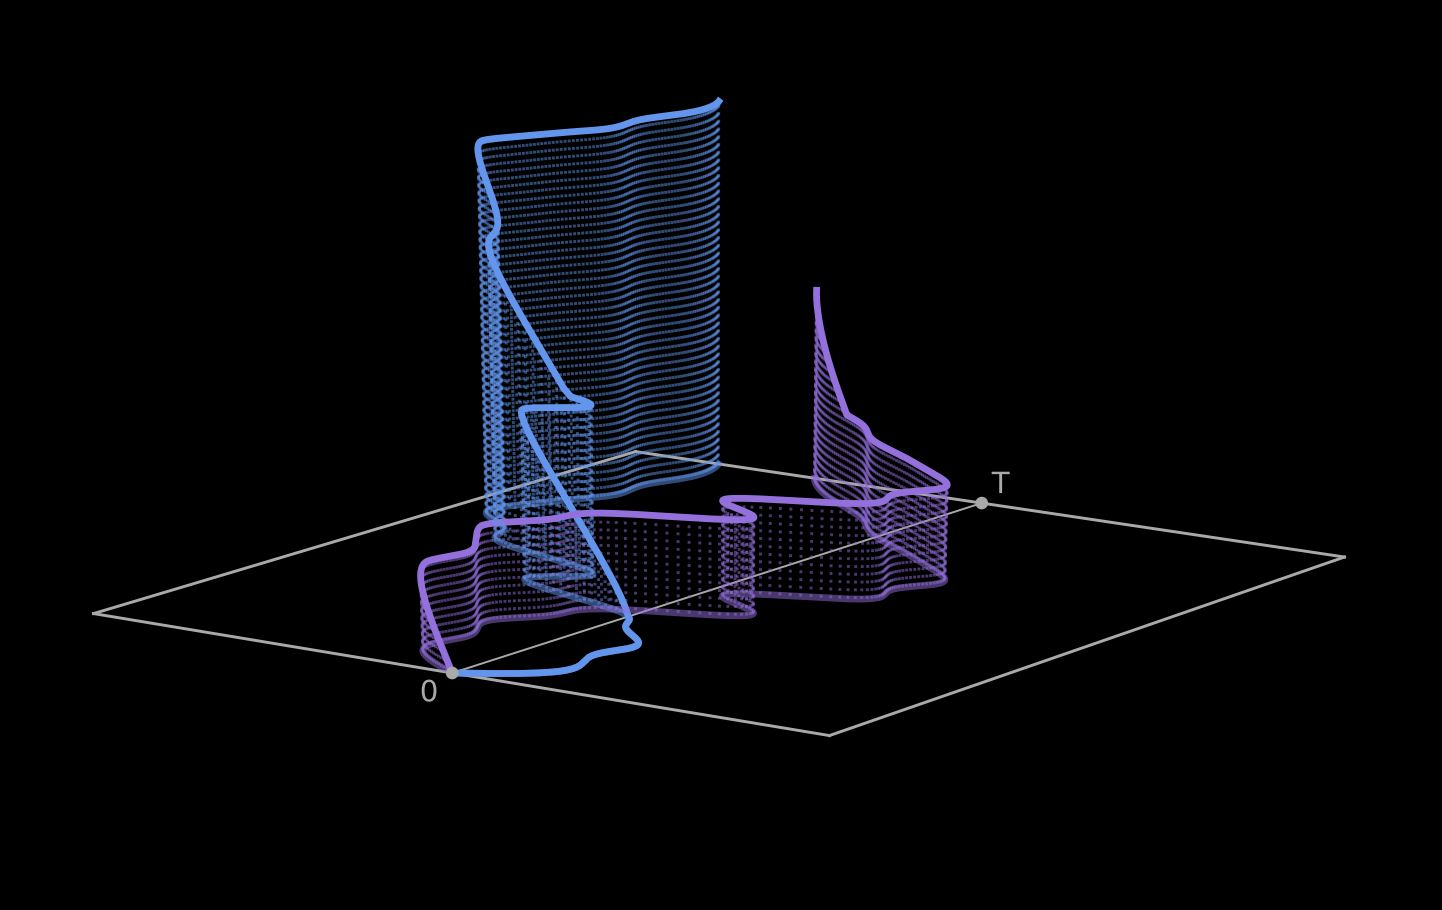
\includegraphics[scale =0.22]{KL/Figures/MaxDouble.JPG}
    %
    \label{fig:max3D}
\end{figure}



%========== Time Average and Integral ===========%
\begin{example} \label{ex:timeIntAvg}
 Consider  the time integral and average of a Brownian path, 
$y_t = 
f(X_t) = \int_0^t x_s\, ds, \ \bar{y}_{t}= 
\bar{f}(X_t) = \frac{1}{t}f(X_t). $
These are clearly centered processes and their covariance kernels of can be found explicitly. Starting with $Y$, 
$$\kappa_{Y}(s,t) =  \left(\int_0^s x_r dr,\int_0^t x_u du \right)_{L^2(\Q)} \overset{\textnormal{Fubini}}{=} \int_0^s\int_0^t \kappa_X(r,u) dr du.$$
A straightforward calculation gives
$\kappa_{Y}(s,t)  = \frac{s^2 t}{2} - \frac{s^3}{6}, \, s\le t.$
%\textbf{Moreover, it is straightforward to show that the eigenvalues are the square of the eigenvalues of Brownian (see Example \ref{ex:KLBM}).}
The covariance function of the time average follows immediately, namely
$\kappa_{\bar{Y}}(s,t)   = \frac{s}{2} -\frac{s^2}{6t}.$
We display in  \Cref{fig:AvgK,fig:IntK} the covariance kernel (top) and first eigenfunctions (bottom) of $f$ and $\bar{f}$, respectively.
The dashed lines in the top panels  are the eigenfunctions of the original (Brownian) path. Note the wider range in the eigenfunctions $F_1,F_2$ for $\bar{f}(X)$ compared to the integrated path for small $t$.  This might come from the greater fluctuations of the time average at inception. 

\end{example}
%========== Maximum ===========%
\begin{example} Consider the running maximum  functional $y_t= 
f(X_t) = \max_{0 \le s \le t} x_s$.  \Cref{fig:max3D} provides an illustration in the $(t,X,Y)$ plane. The mean function is in this case non-zero and$-$using, e.g., the reflection principle$-$given by $\E^{\Q}[y_t] = \sqrt{\frac{2}{\pi} t}$. The covariance kernel admits an explicit yet complicated expression \cite{Benichou}, 
$$\kappa_Y(s,t) = \frac{s}{2} + \frac{\sqrt{s(t-s)}-2\sqrt{st} + t \arcsin(\sqrt{s/t})}{\pi}, \quad s \le t.$$
\Cref{fig:MaxK} displays the covariance kernel (top) and first eigenfunctions (bottom). The latter turns out to be quite close to the eigenfunctions of Brownian motion. 

\end{example}



\begin{figure}[t]%[H]
%\centering
\caption{Covariance kernels (top) and eigenfunctions (bottom).}
\vspace{-4mm}
\begin{subfigure}[b]{0.32\textwidth}
    \centering
    \caption{Time average}
    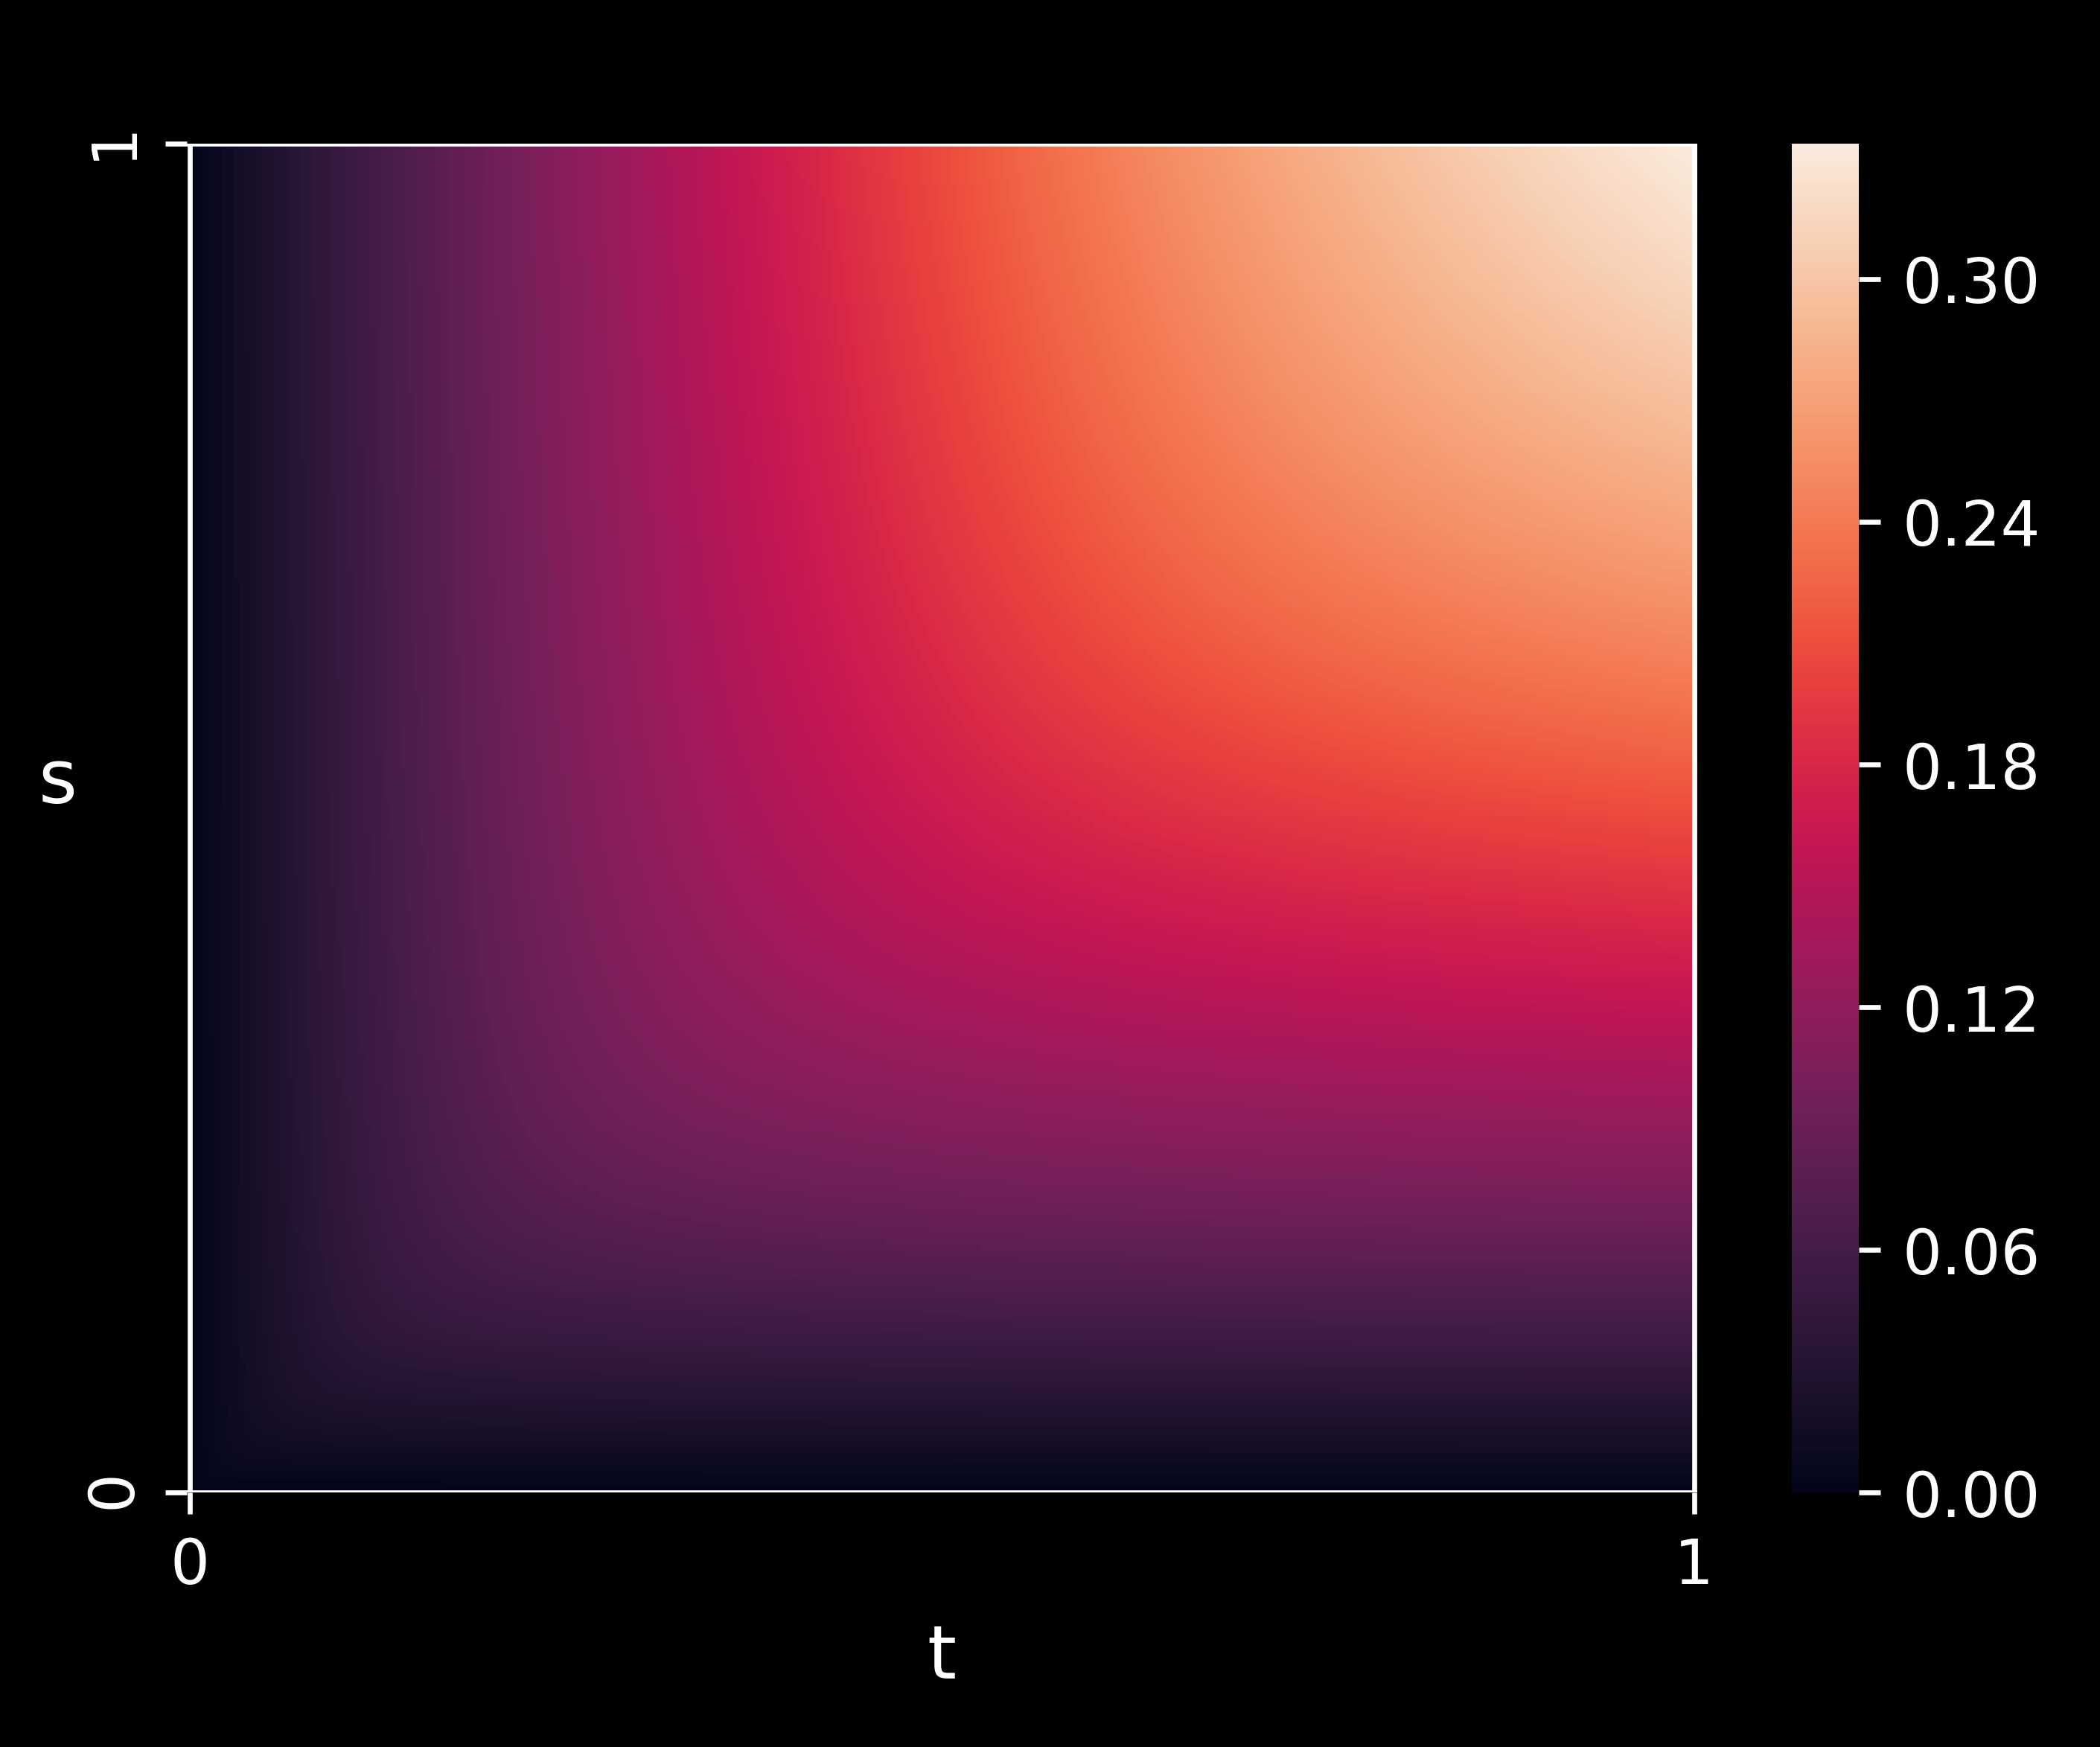
\includegraphics[scale =0.38]{KL/Figures/KLAverageKernel.png}
    \label{fig:AvgK}
\end{subfigure}
\begin{subfigure}[b]{0.32\textwidth}
    \centering
    \caption{Time integral}
    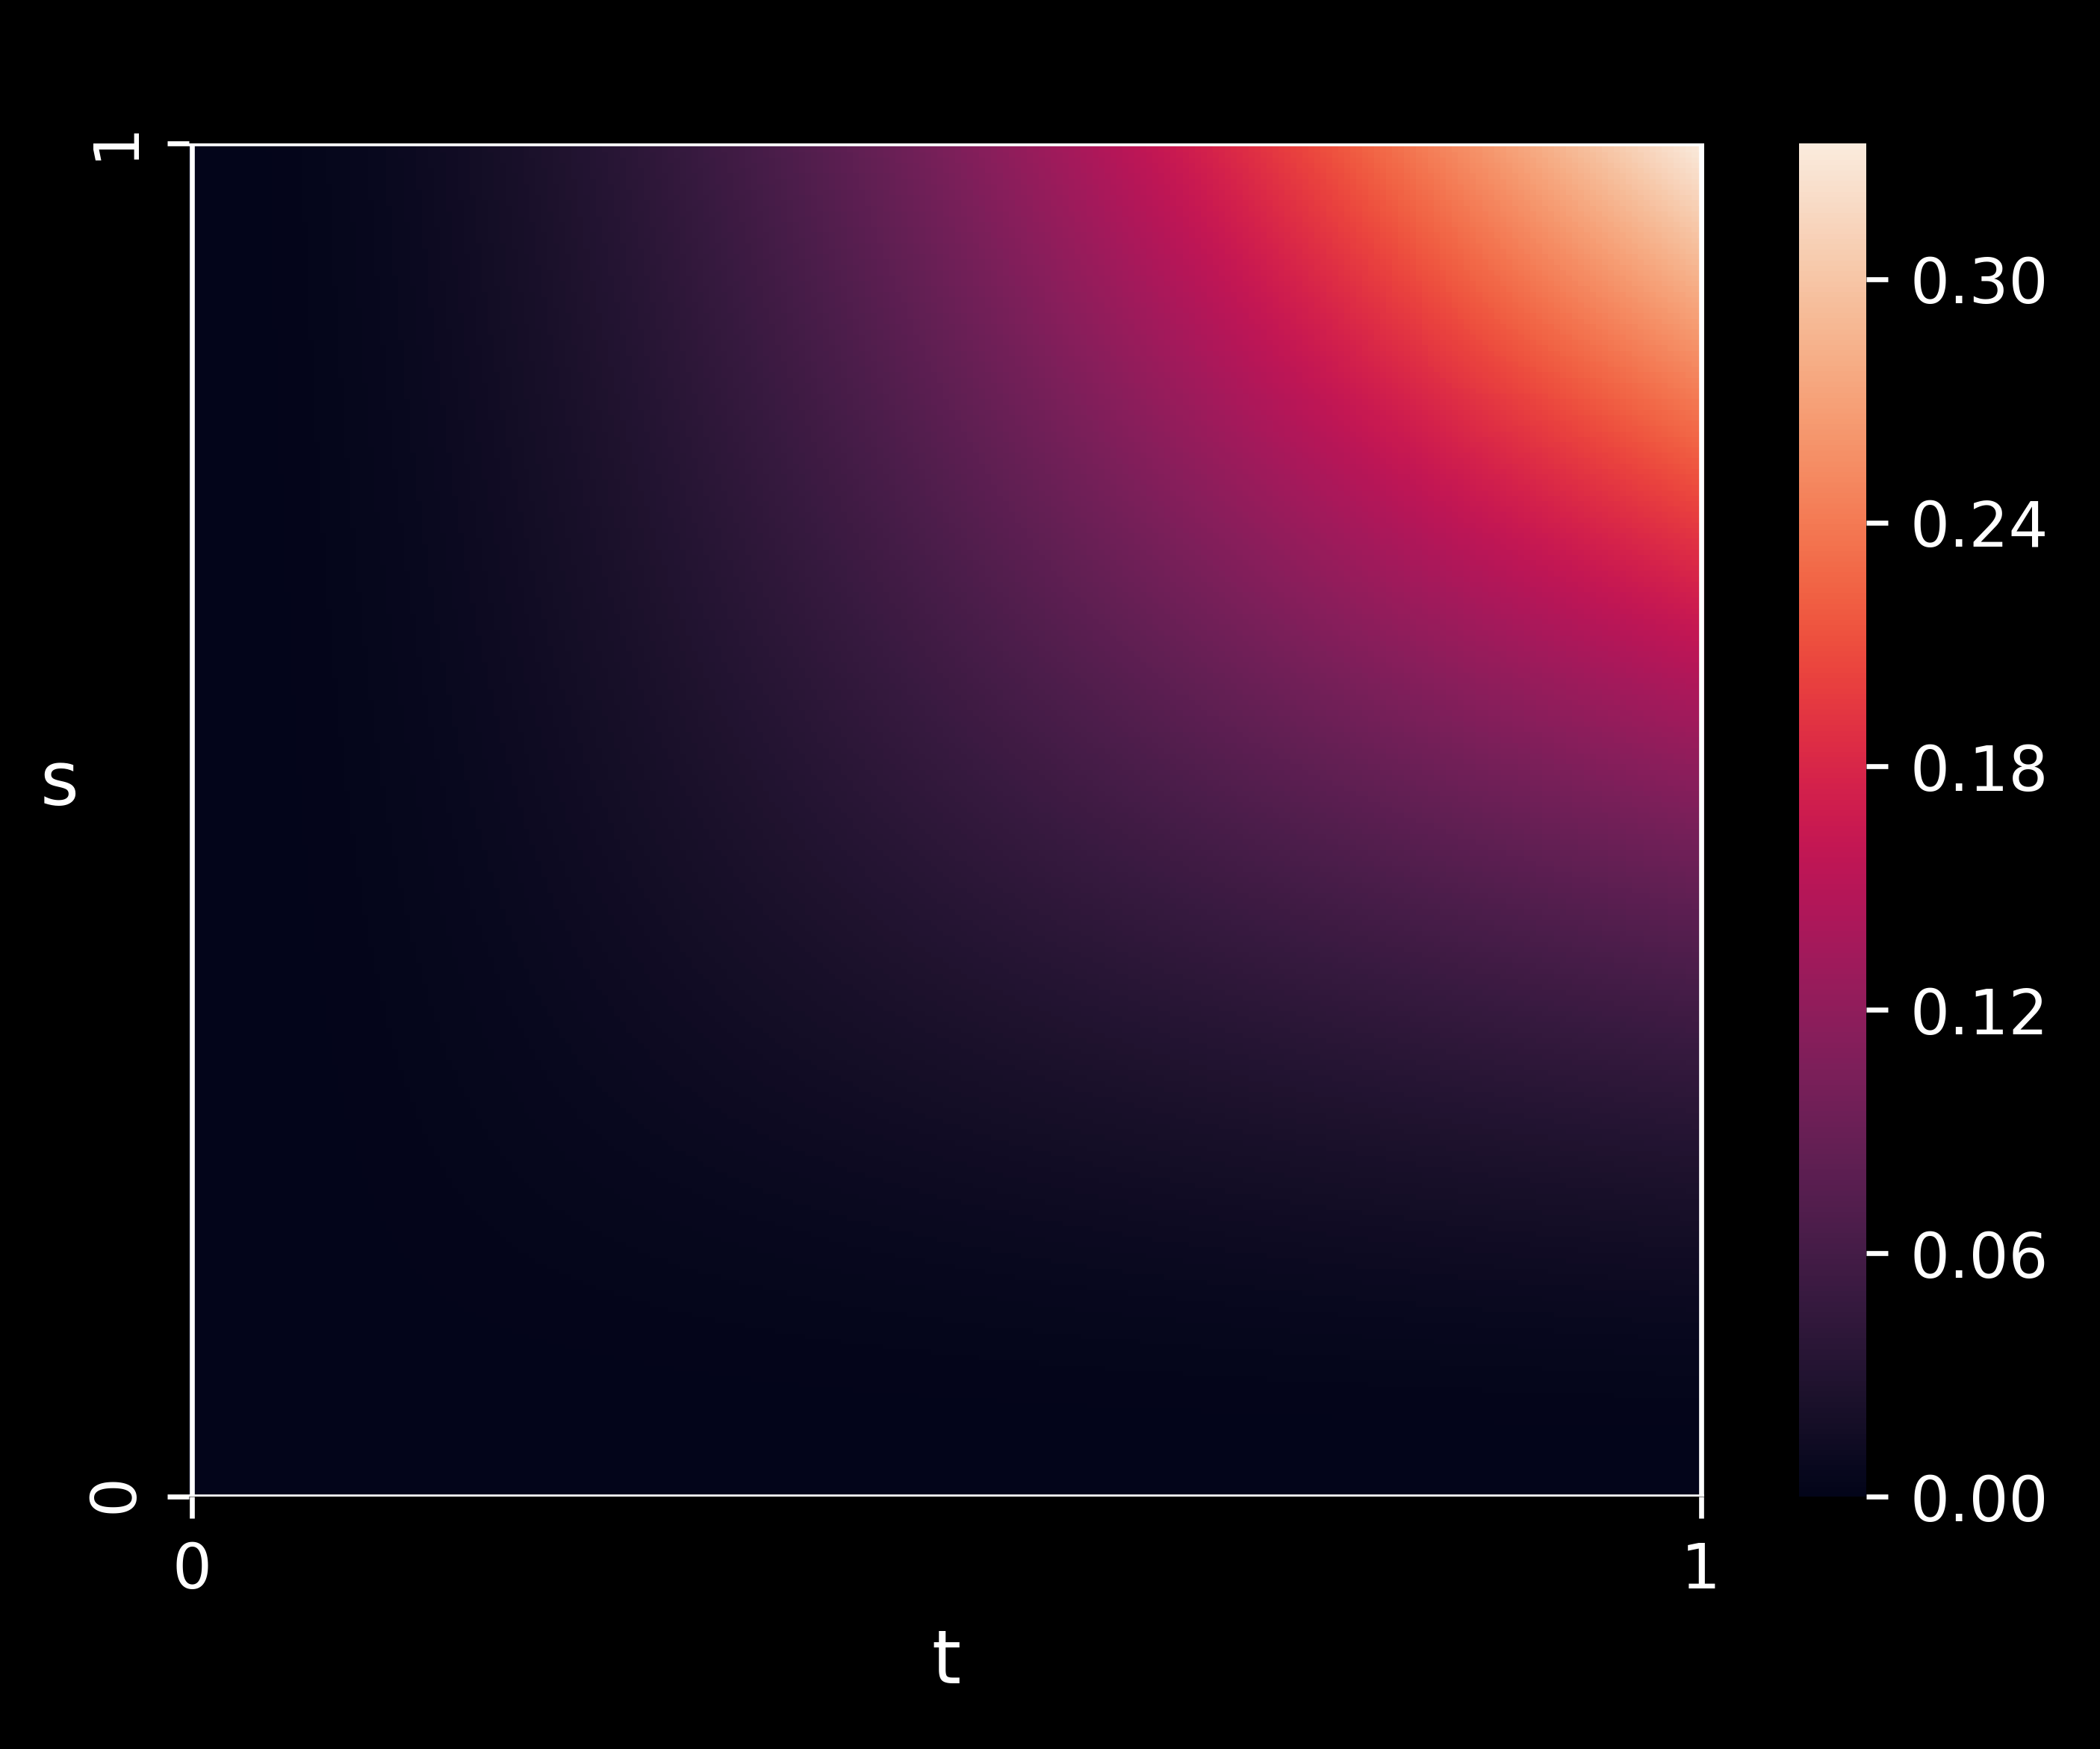
\includegraphics[scale =0.38]{KL/Figures/KLIntegralKernel.png}
    \label{fig:IntK}
\end{subfigure}
\begin{subfigure}[b]{0.32\textwidth}
    \centering
    \caption{Running maximum}
    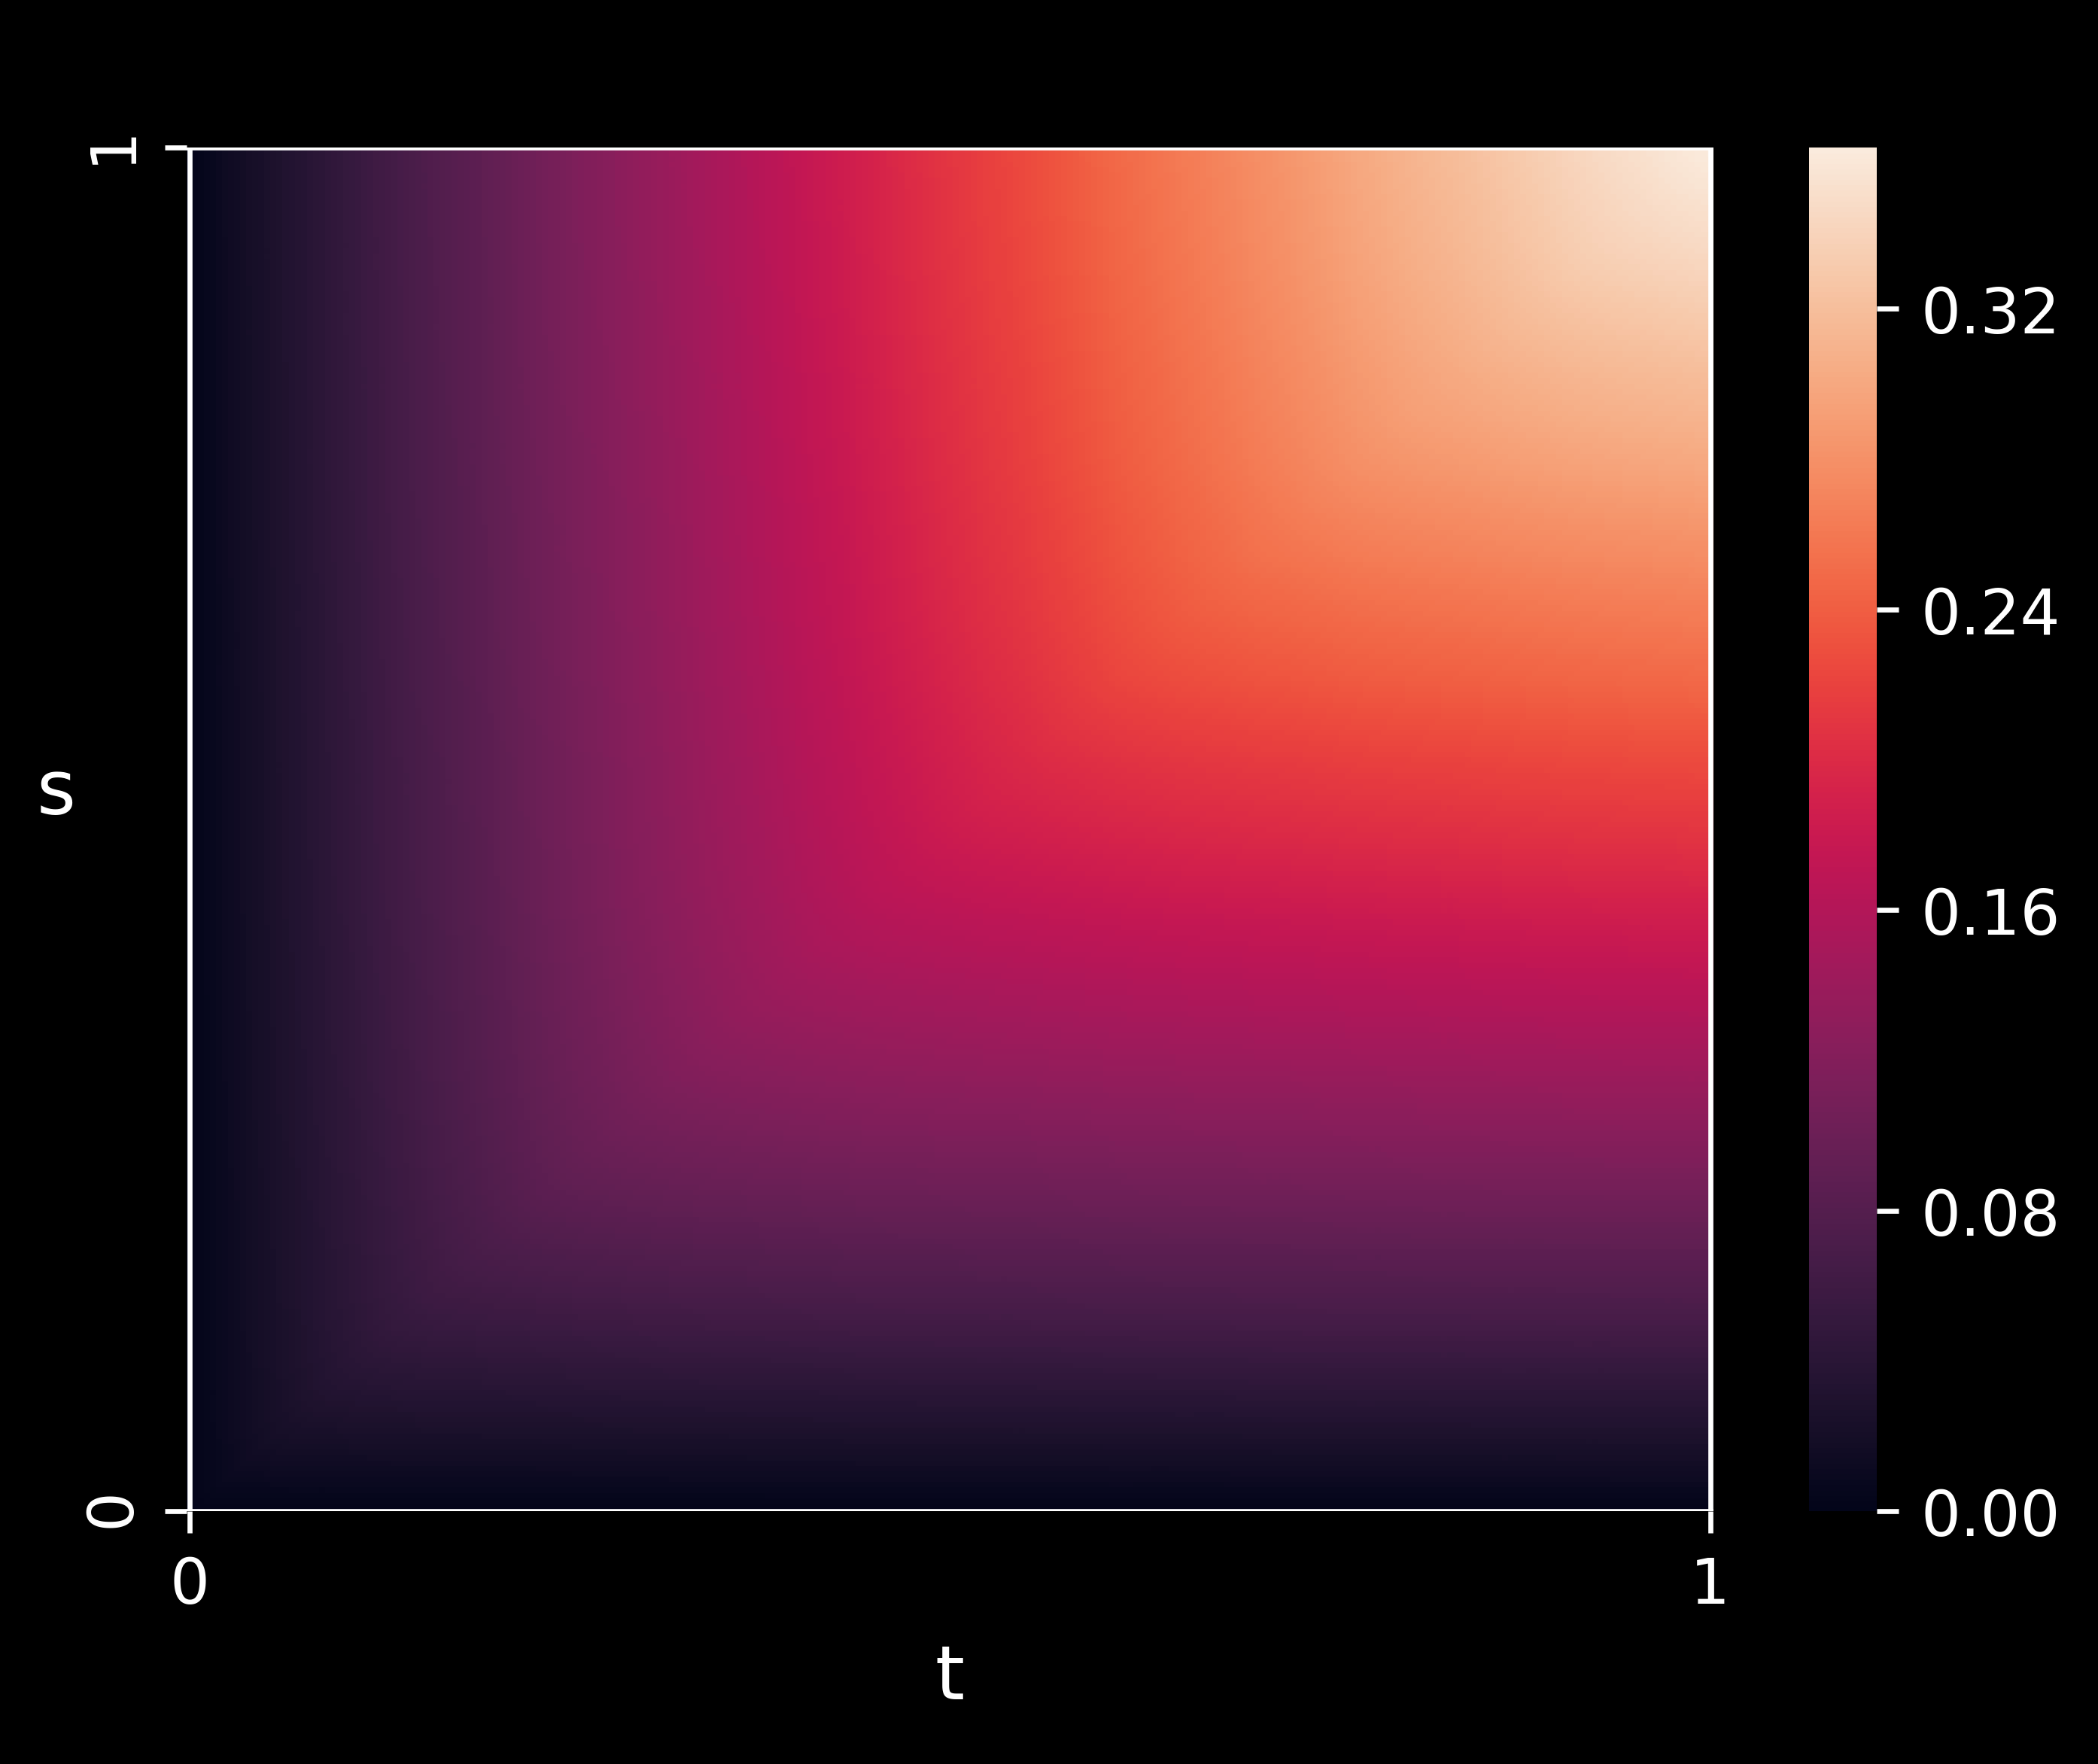
\includegraphics[scale =0.38]{KL/Figures/KLMaximumKernel.png}
    \label{fig:MaxK}
\end{subfigure}
\vspace{2mm}

%\centering
\begin{subfigure}[b]{0.32\textwidth}
    \centering
    %\caption{Time average}
    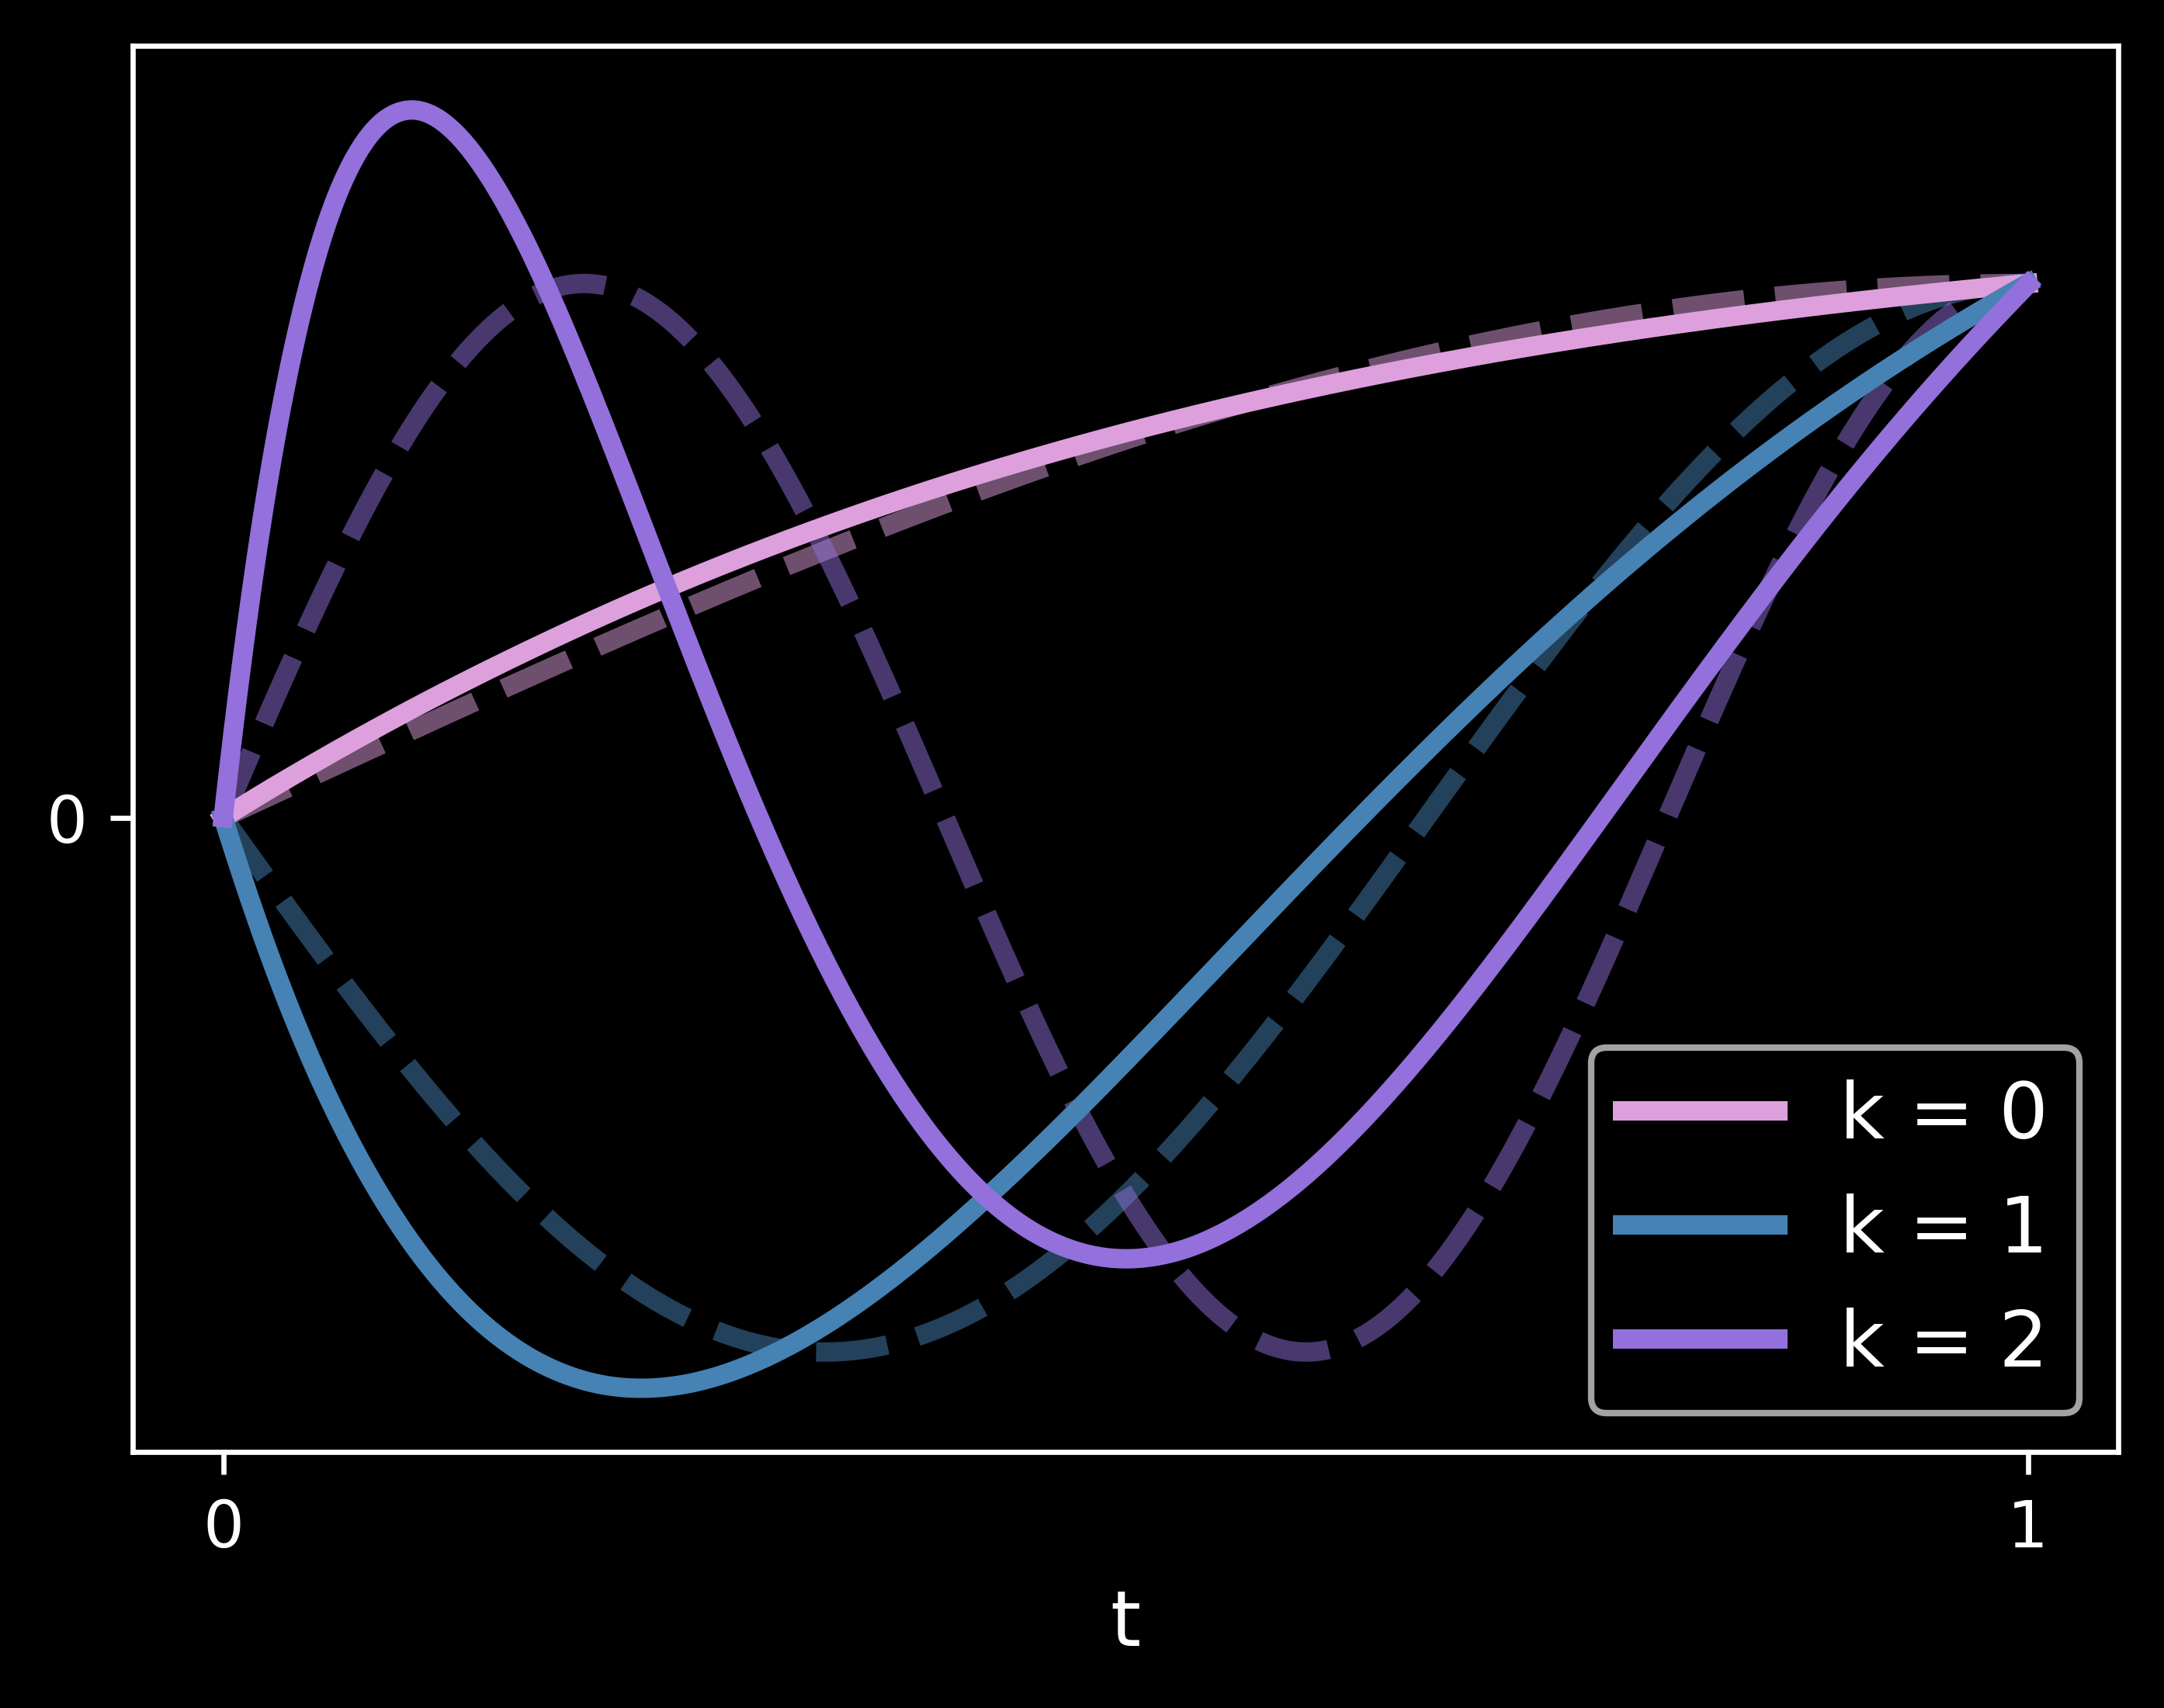
\includegraphics[scale =0.385]{KL/Figures/KLAsian.png}
\end{subfigure}
\begin{subfigure}[b]{0.32\textwidth}
    \centering
    %\caption{Time integral}
    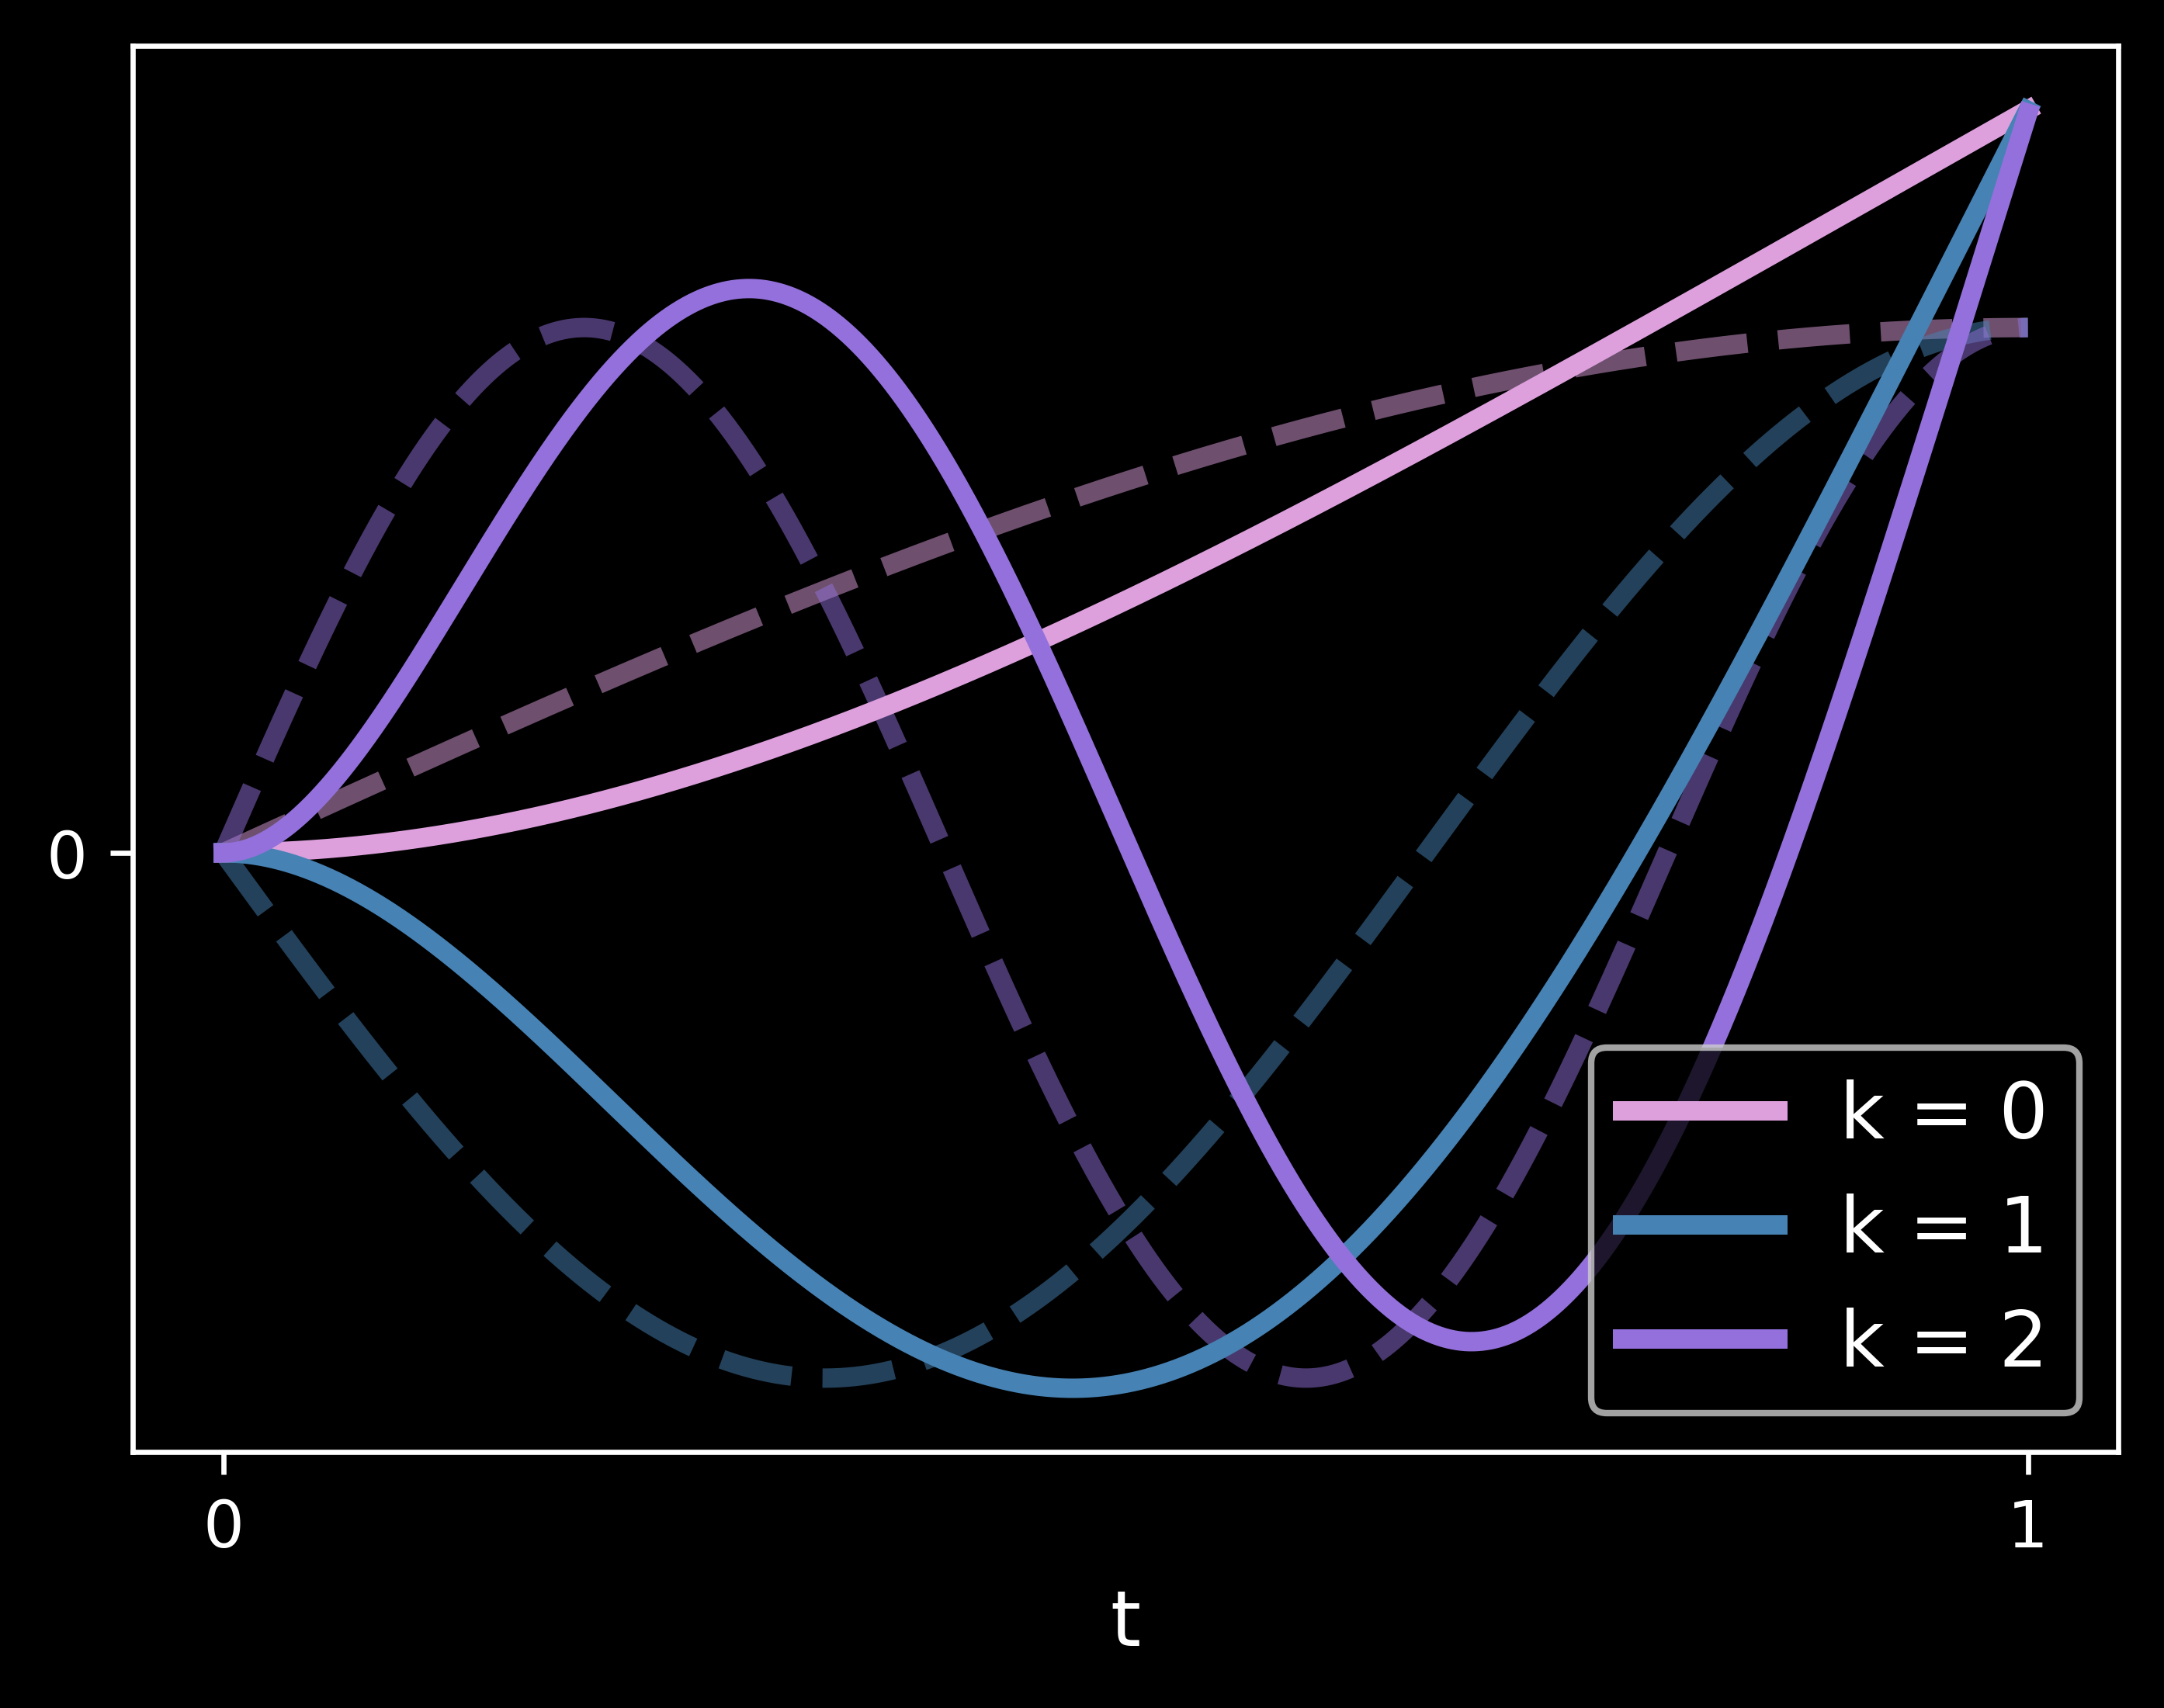
\includegraphics[scale =0.385]{KL/Figures/KLIntegral.png}
\end{subfigure}
\begin{subfigure}[b]{0.32\textwidth}
    \centering
    %\caption{Time integral}
    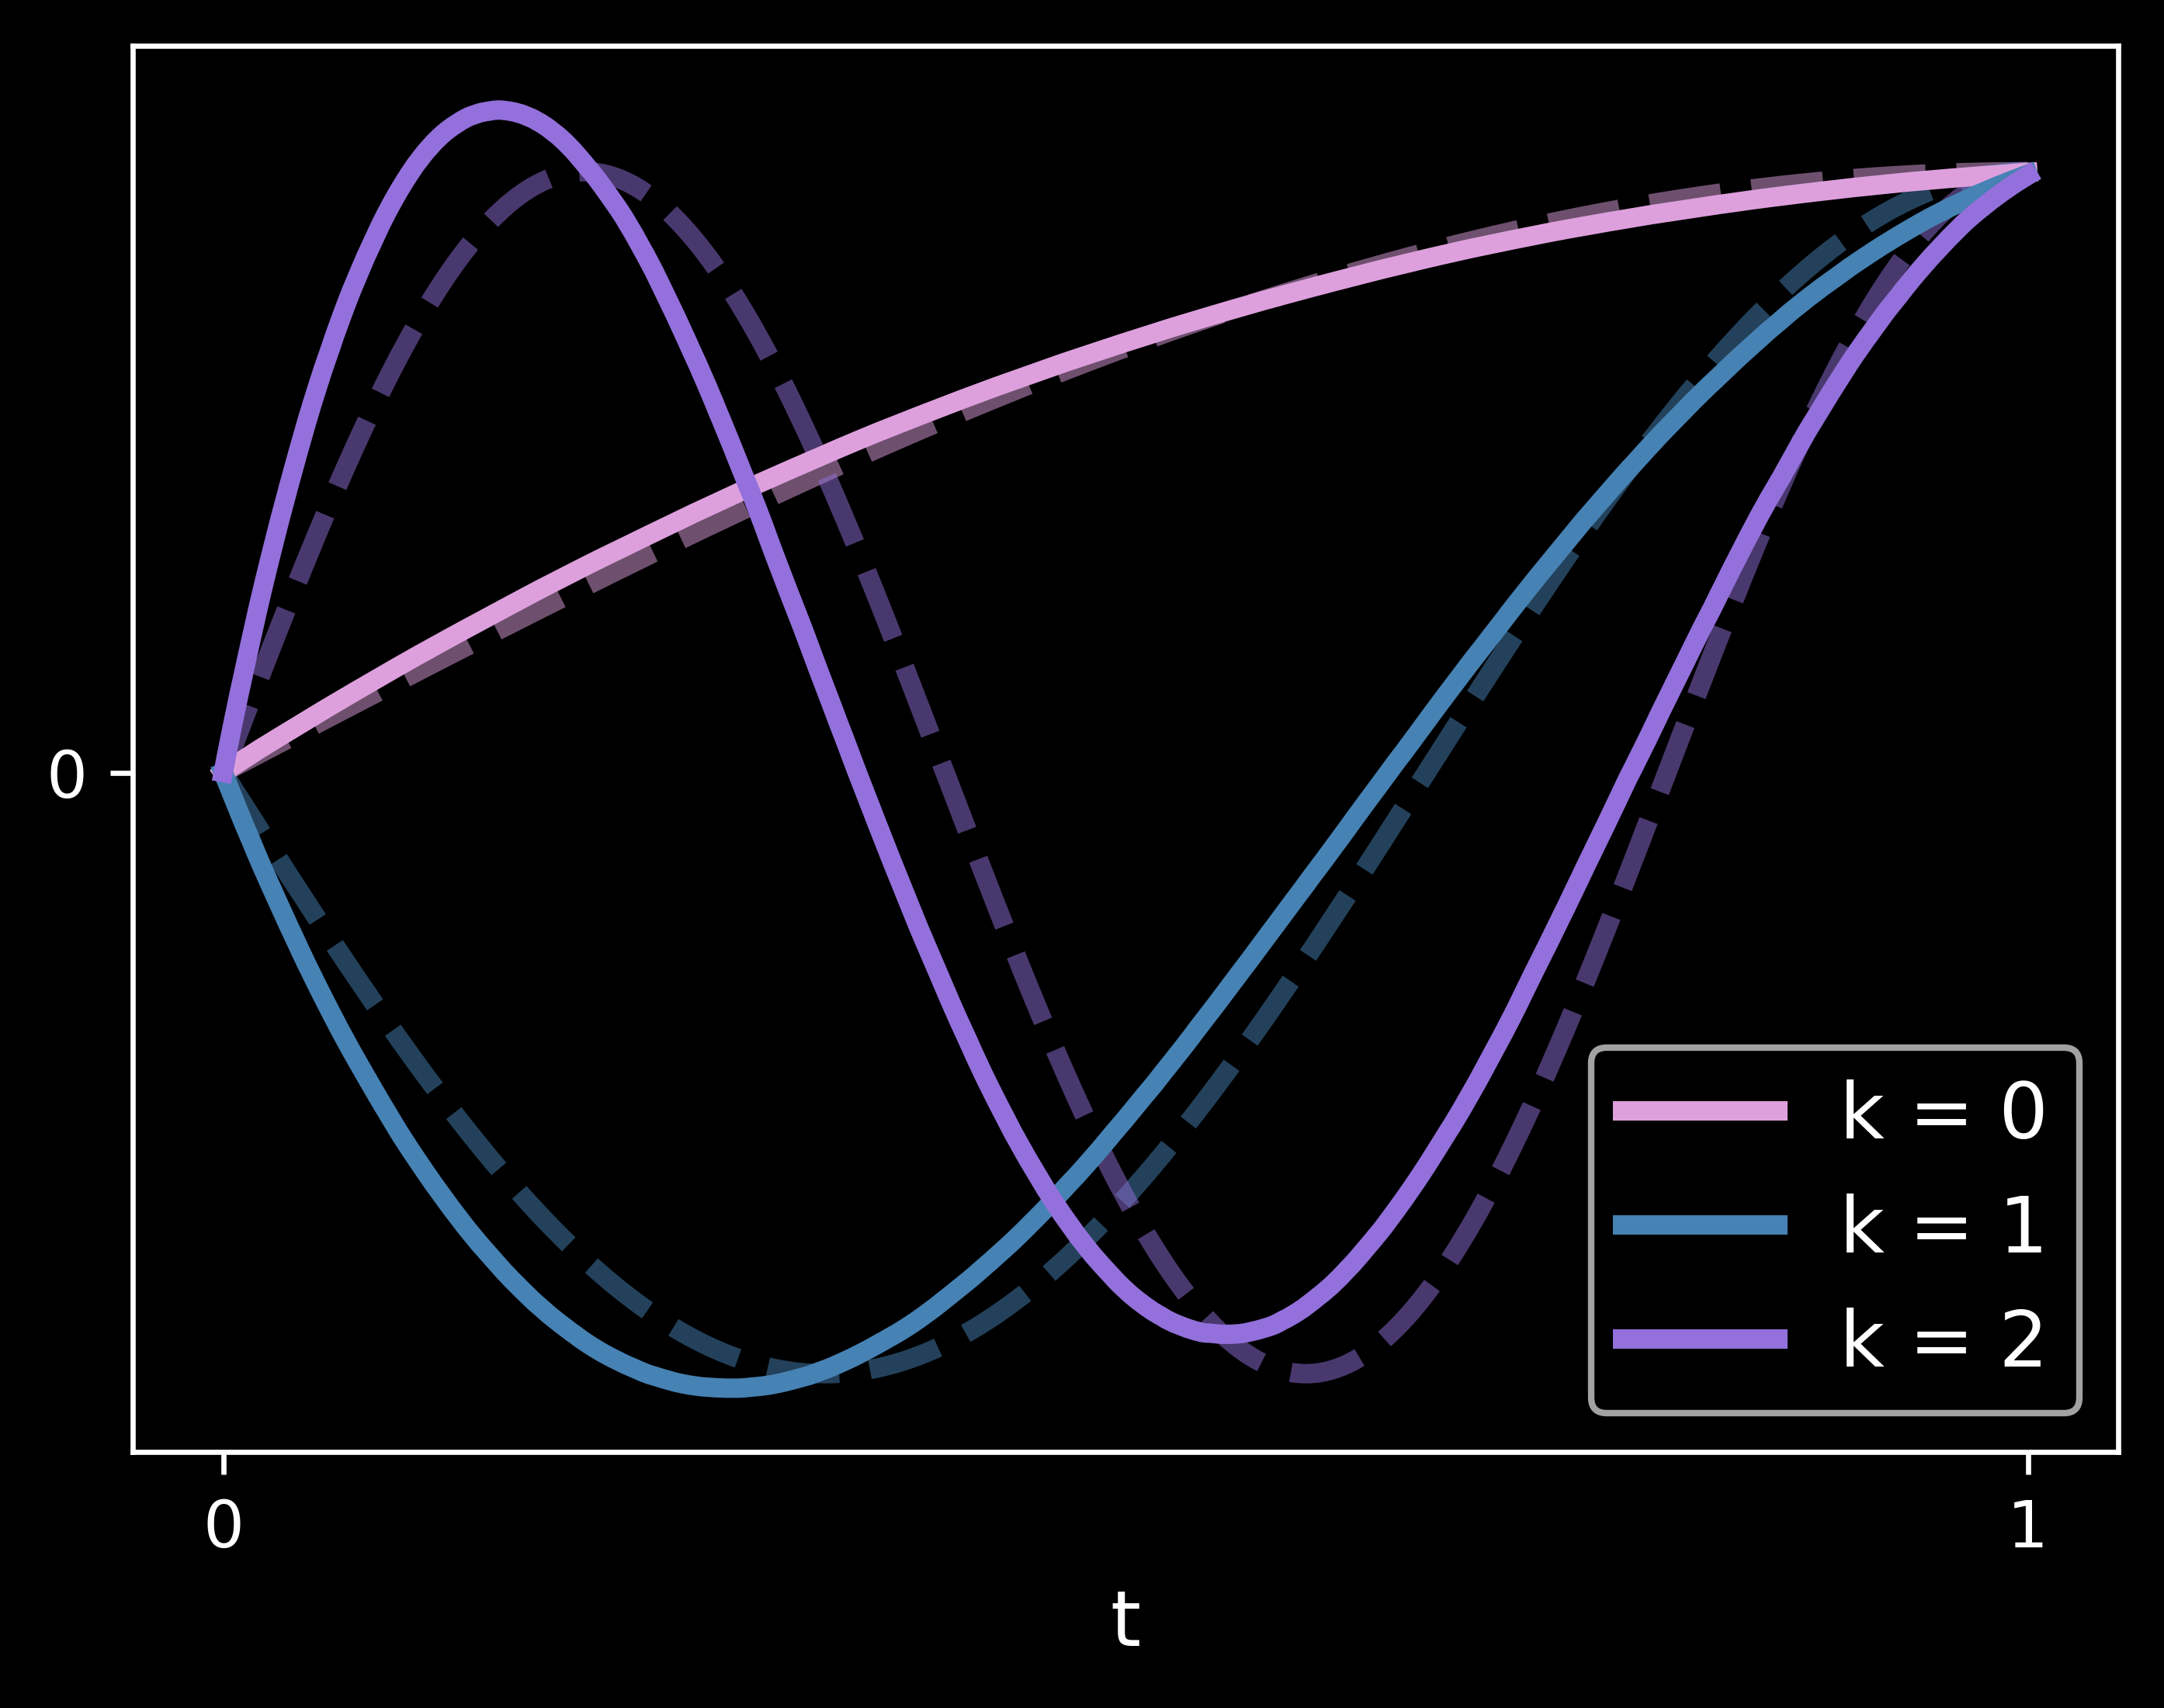
\includegraphics[scale =0.38]{KL/Figures/KLLookback.png}
\end{subfigure}
\vspace{1mm}
\begin{center}
    \footnotesize{
    \textit{Solid lines: transformed
     path.  Dashed lines: Brownian motion.}}
\end{center}
\vspace{-3mm}
\end{figure}

\subsection{Numerical Results} \label{ssec: numResult}
Let us compare the $L^2(\Q \otimes \, dt)$ error  
$\lVert Y^{K,\frakF} - Y \rVert^2_{*} $ in the Brownian case for the two avenues discussed at the beginning of this section. When $Y^{K,\frakF} = (f \circ \pi^{K,\frakF})(X) $, the error is calculated using Monte Carlo simulations. As in  \Cref{sec:numResultX}, we choose $T=1$, $N=10^4$ and $K\in \{1,\ldots,128\}$.  
\Cref{fig:L2Error} displays the result for the running maximum, integral and average functionals. We also add the Brownian motion itself, corresponding to the identity functional $f(X)=X$. We observe a clear improvement when projecting the transformed path. Moreover, it comes as no surprise that smooth functionals (integral, average) exhibits a faster rate of convergence than the running maximum, highly sensitive to local behaviours of a path. 

\begin{figure}%[H]
    \centering
    \caption{$L^2(\Q \otimes dt)$ approximation errors. }
    \vspace{-2mm}
    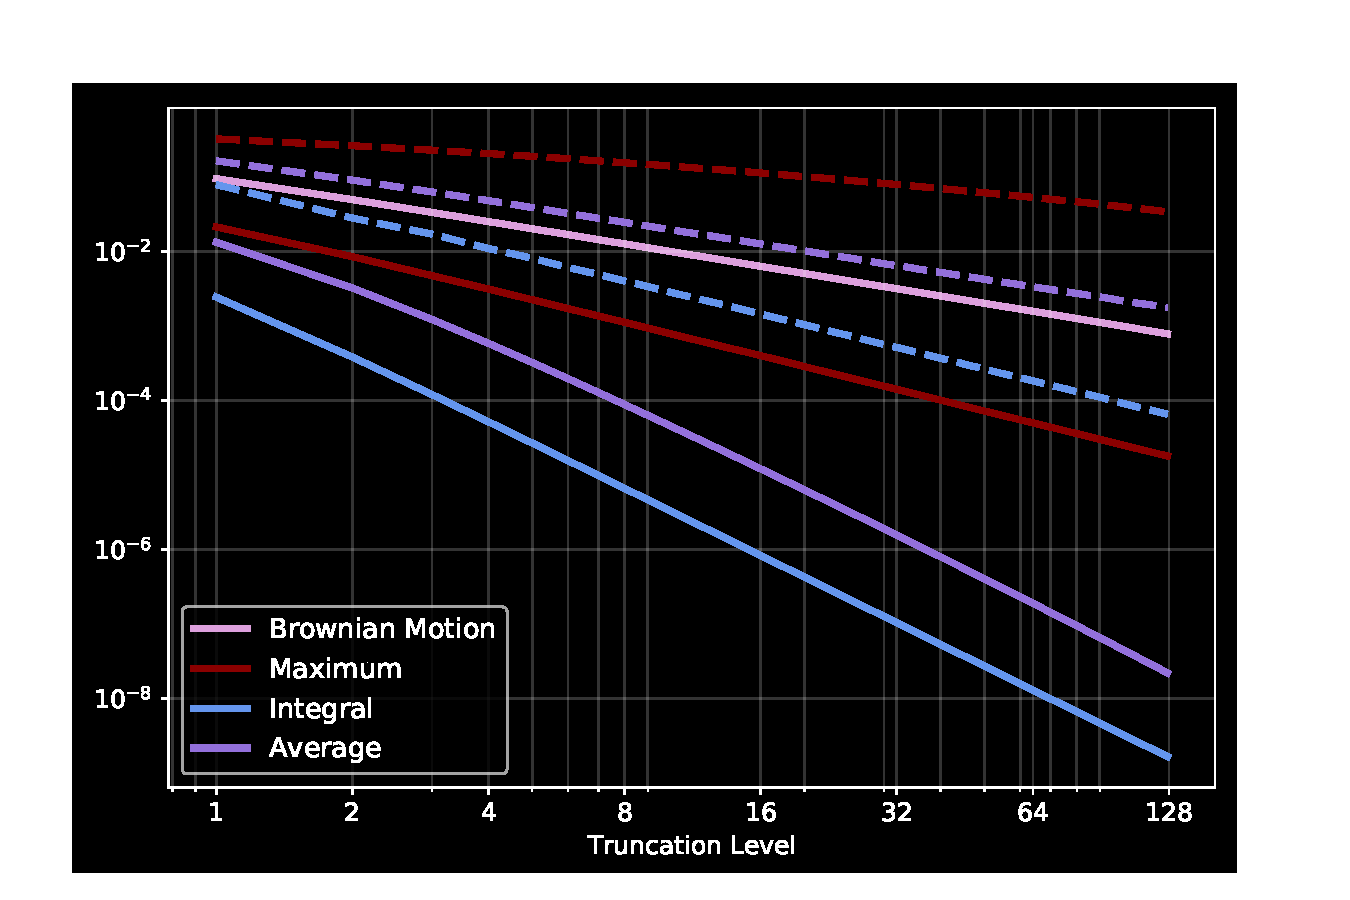
\includegraphics[scale =0.38]{KL/Figures/Error_nSim5000_N1000.pdf}
    \label{fig:L2Error}
    \\
    
    \vspace{1mm}
    
    \footnotesize{
    \textit{Dashed lines: functionals of projected paths. \\Solid lines: projected functionals.}}
\end{figure}

% \subsection{Monotone Convergence}
% When do we have $f_K \nearrow f$? This would ensure, in particular, that 
% $$\lim_{K\to \infty} \E^{\Q}[f_K(X_T)] = \E^{\Q}[f(X_T)].$$ 

% \begin{example}
% (\textbf{Running maximum}) Take 
% $f_K = f \circ \pi^{K,\frakF}$, where $\frakF$ are the Schauder functions and $\calH = \calR$. Then increasing the order $K$ adds new vertices on the graph of $x^{K,F}$ while keeping the ones already there. Hence the maximum, attained on a vertex can only increase. In other words, 
% $$f_K(X_t) = \max_{s\, \le t} x_s^{K,\frakF} = \max_{t_n\, \in \, \Pi_K} x_{t_n}^{K,\frakF} \le \max_{t_n\, \in \, \Pi_{K'}} x_{t_n}^{K',\frakF} = f_{K'}(X_t),
% $$
% if $\Pi_K$ denotes the $K-$th dyadic partition. 

% \end{example}



\subsection{Discussion: Projection of Functionals using the Signature} \label{sec:sigFunc}

Another approximation of $Y=f(X)$ can be obtained by combining  signature functionals in a linear fashion. For instance, one can consider all the words of length less than $\bar{K} \in \N$, giving the approximation
  \begin{equation}\label{eq:sigPayoff}
      y^{K,\calS}_t := \sum_{l(\alpha)\, \le \, \bar{K}} \xi^f_{\alpha} \calS_{\alpha}(X_t), 
  \end{equation}
  \vspace{-3mm}
  
  with $K = |\{\alpha \, | \, l(\alpha)\le \bar{K}\}|=2^{\bar{K}+1}-1.$
  The coefficients $\xi^f_{\alpha}$ may depend on  $X_0$  only and can be  calculated by either regressing  $Y$ against the signature elements or using a Taylor formula for functionals; see \cref{chap:Taylor}.  %\cite{LittererOberhauser} when $f$ is smooth (in the Dupire sense) and $X$ is a diffusion. 
    % In the literature,   $\eqref{eq:sigPayoff}$ is referred to  as  \textit{polynomial functional}  \cite{LittererOberhauser} or \textit{signature payoff} \cite{Szpruch,LyonsNum} in finance. 
     
     The appeal of such projection comes from the fact that polynomial functionals are dense in the space of continuous functionals restricted to  paths of bounded variation; see Theorem 5 in  \cite{LittererOberhauser}.  
     On the other hand, despite the existence of   packages to calculate the signature of discrete time paths (e.g., \texttt{iisignature} and \texttt{esig} in Python), the projection in $\eqref{eq:sigPayoff}$ is still  challenging from a computational perspective. 
     Indeed, contrary to the reconstruction in  \Cref{sec:sigLegendre}, the signature functionals have to be known at \textit{every} intermediate time. Also, as there is a priori no recipe to select words up to a given length,  we must retain all of them so the number of elements doubles every time a layer is added. 

